\documentclass[11pt]{article}    
    \addtolength{\topmargin}{-3cm}
    \addtolength{\textheight}{3cm}
\usepackage{graphicx}
\usepackage[section]{placeins}
\usepackage{geometry}
\usepackage{color,soul}
\usepackage{pdfpages}
\usepackage[noae]{Sweave}
\usepackage{quoting}
\usepackage{lipsum}
\usepackage{•} 



\title{Revised Alert Messages Application}
\author{Peter Higgins, PhD}
\date{April 25, 2022}

\begin{document}
\maketitle




\section{Introduction}

This work is the latest revision of previous versions that implements changes requested by the project specialist, Elizabeth Waagen, AAVSO, including:

\begin{enumerate}
	\item Add forum links to notice input and html document.     
    \item Automate handling of include graphic in original and edited submittals.    
    \item Reorder star table columns, vertically.    
    \item Cosmetic changes, fix errors.
    
\end{enumerate}   

\section{Staff member menu}
Annum has been changed to ANnum, shown circled in red.
\begin{figure}[hbtp]
\centering
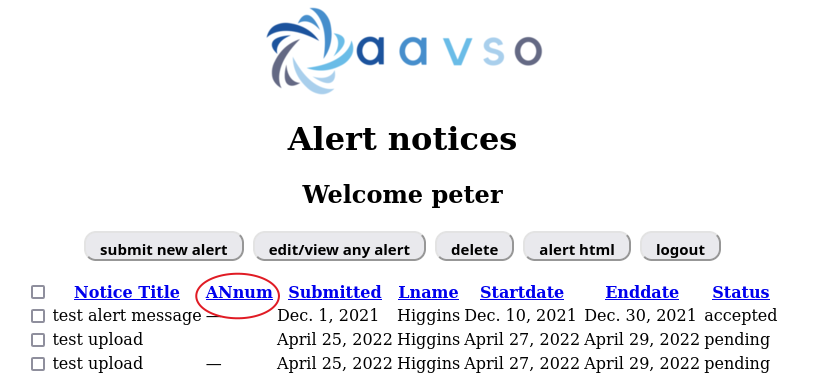
\includegraphics[scale=1]{menu1.png}
\caption{staff menu}
\end{figure}

\section{Changes in staff edit/view of a notice}
Several changes have been made including:
\begin{enumerate}
	\item This form still allows staff to enter a new notice because often a notice is entered by staff from email information from PIs. This probably will still be the case even when PI's can use this app to enter notices directly.
	\item The form is 30 margin pixels from left side of page, not centered. Title is changed. This is consistent with Sara's specification for sun spot entry.   
    \item An entry box has been added for staff entry only of the AAVSO relevant forums (red ellipse). Staff can cut and paste forum string data giving title and html link, but the leading character before title and link must be a \# charater instead of a dash character as shown by blue ellipse.   
		\item Entry of an optional graphic is uses a  forms.FileField control in the form, shown here within a green ellipse, and a model.CharField  as before. The handling of this entry has been changed. When a new notice is created, including an optional graphic is optional and the notice can be generated and saved to the database without it. No error is thrown if no graphic is chosen. But if a graphic is entered, several things happen: the graphic is now saved in the table field in the database AND it is now automatically uploaded into the project so it is found by the html writer. When selected its name appears alongside the control on the entry form. But unlike all other fields, it does not appear in an edit of this notice, even though it is in the database and has been uploaded. That is when the notice is called back by an edit, the edit doesn't include the original selection. Because of this, previous versions of this app required the user to reselect it even when it doesn't change in the edit. This is a problem because the editor may not remember what was originally selected, and it doesn't show on the form. This revision includes a work-around to this problem. Now when a notice record is selected by the checkbox, the included file (if this one) is captured using REQUEST.POST and stored in a session variable. When the edit is saved if no new selection is discovered, the previous selection is recalled from the session variable and the revised notice record is updated with the previous selection (so the user now does nothing to restore the original choice). The code for this complication is in two funtions - the new notice handler, and the edit notice handler shown in the figures below.   
	\item Figure 3 shows the bottom of the new or edit form. It is moved to the left and the entries are not centered as highlighted by green ellipse. As requested the star columns now are arranged vertically not horizontally so that s2 is below s1 in the left column, not beside s1 in the right column (black ellipse). 
\end{enumerate}   



\begin{figure}[hbtp]
\centering
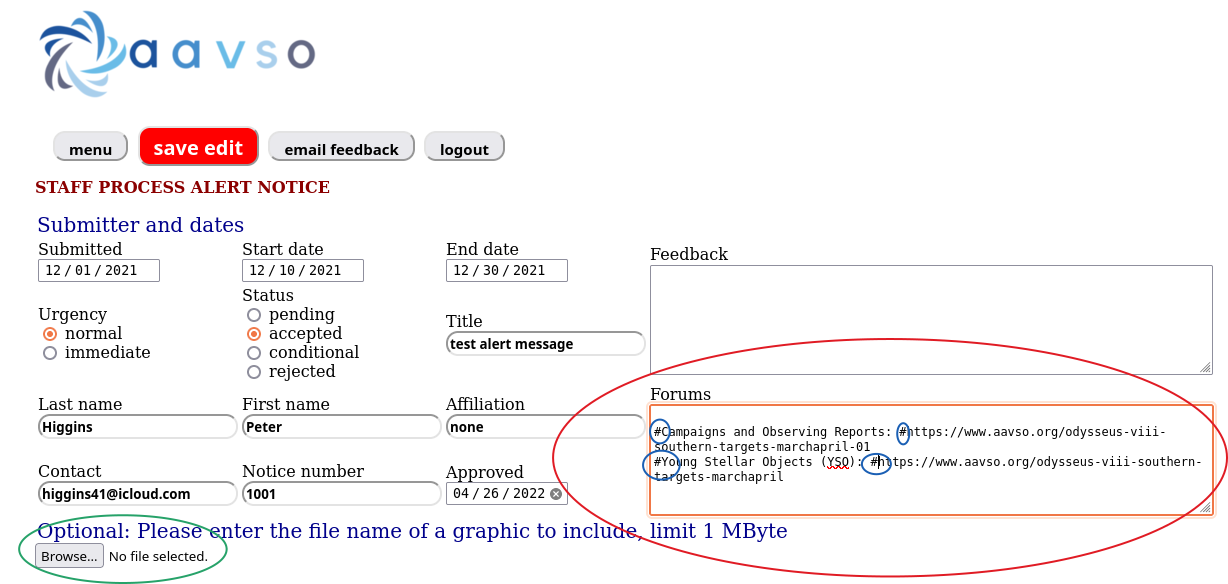
\includegraphics{edittop.png}
\caption{Revised new entry form, top
}
\end{figure}


\begin{figure}[hbtp]
\centering
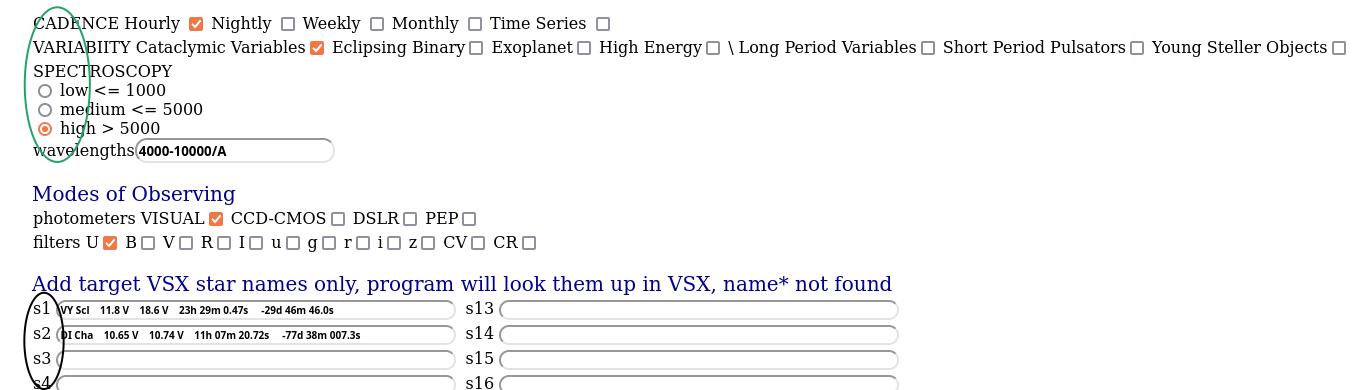
\includegraphics[scale=1.0]{editbottom.png}
\caption{Revised new entry form, bottom}
\end{figure}

The code for processing the include graphic is:

\end{document}
